\documentclass[10pt]{article}
\usepackage[polish]{babel}
\usepackage[utf8]{inputenc}
\usepackage[T1]{fontenc}
\usepackage{amsmath}
\usepackage{amsfonts}
\usepackage{amssymb}
\usepackage[version=4]{mhchem}
\usepackage{stmaryrd}
\usepackage{graphicx}
\usepackage[export]{adjustbox}
\graphicspath{ {./images/} }

\title{KLASY PIERWSZE I DRUGIE }

\author{}
\date{}


\begin{document}
\maketitle
\begin{enumerate}
  \item Odcinek \(A B\) ślizga się po ramionach kąta prostego w ten sposób, że punkt \(A\) należy do jednego ramienia, a punkt \(B\) do drugiego. Jaki kształt będzie miała droga, którą przebędzie środek odcinka \(A B\). Odpowiedź uzasadnij.
  \item Czworokąt wypukły podzielono na cztery części łącząc środki jego boków jak na rysunku. Wykaż, że suma pól części zacienionych jest równa sumie pól części niezacienionych.
  \item Wykaż, że w trójkącie \(A B C\) dwusieczna kąta \(A C B\) i symetralna boku \(A B\) przecinają się na okręgu opisanym na tym trójkącie.\\
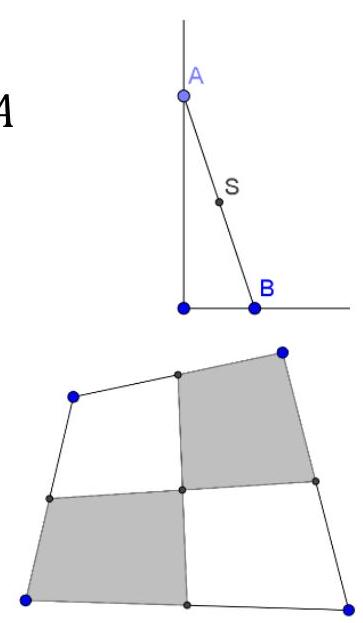
\includegraphics[max width=\textwidth, center]{2024_11_21_219d6f5dddf91235b0b5g-1(1)}
\end{enumerate}

\section*{KLASY TRZECIE}
\begin{enumerate}
  \item Trójkąt prostokątny \(A B C\) ślizga się po ramionach kąta prostego w ten sposób, że punkt \(A\) należy do jednego ramienia, a punkt \(B\) do drugiego. Jaki kształt będzie miała droga, którą przebędzie wierzchołek kąta prostego \(C\). Odpowiedź uzasadnij.
  \item Czworokąt wypukły podzielono na dziewięć części dzieląc każdy bok na trzy równe części i łącząc punkty podziału jak na rysunku. Wykaż, że suma pól części czerwonych jest równa sumie pól części niebieskich. Uwaga! Nie jest oczywiste, że wszystkie odcinki łączące punkty na przeciwległych bokach zostały podzielone na trzy równe części.\\
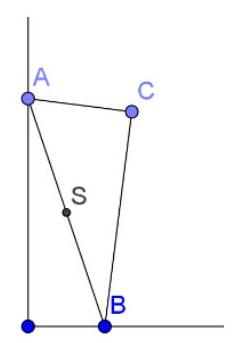
\includegraphics[max width=\textwidth, center]{2024_11_21_219d6f5dddf91235b0b5g-1}
  \item Rozwiąż układ równań:
\end{enumerate}

\[
\left\{\begin{array}{l}
a^{2}+2=2 a+b \\
b^{2}+2=2 b+c \\
c^{2}+2=2 c+d \\
d^{2}+2=2 d+e \\
e^{2}+2=2 e+a
\end{array}\right.
\]


\end{document}